\title{API}

{{navbar}}

Edward's design reflects the building blocks for probabilistic
modeling. It defines interchangeable components, enabling rapid
experimentation and research with probabilistic models.

Edward is named after the innovative statistician
\href{https://en.wikipedia.org/wiki/George_E._P._Box}{George Edward
Pelham Box}. Edward follows Box's philosophy of statistics and machine
learning \citep{box1976science}.

First gather data from some real-world phenomena. Then cycle through
\href{http://www.annualreviews.org/eprint/7xbyci3nwAg5kEttvvjk/full/10.1146/annurev-statistics-022513-115657}
{Box's loop} \citep{blei2014build}.

\begin{enumerate}
\item Build a probabilistic model of the phenomena.
\item Reason about the phenomena given model and data.
\item Criticize the model, revise and repeat.
\end{enumerate}

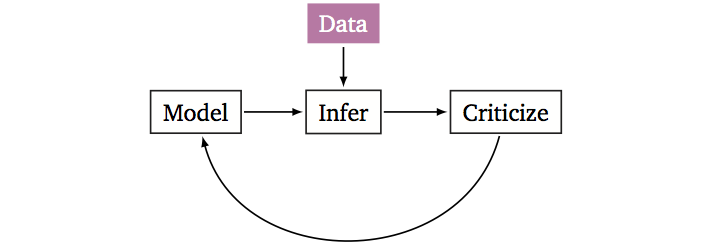
\includegraphics{/images/model_infer_criticize.png}

Here's a toy example. A child flips a coin ten times, with the set of outcomes
being \texttt{{[}0,\ 1,\ 0,\ 0,\ 0,\ 0,\ 0,\ 0,\ 0,\ 1{]}}, where \texttt{0}
denotes tails and \texttt{1} denotes heads. She is interested in the probability
that the coin lands heads. To analyze this data, she first needs to build a
model: suppose she assumes the coin flips are independent and land heads with
the same probability. Second, she must reason about the phenomenon: this
means using an algorithm to infer the model given data. Finally, she should
criticize the model: analyze whether the model captures the real-world
phenomenon of coin flips. If it doesn't, then she may revise the model and
repeat.

Navigate modules enabling this analysis above.

\subsubsection{References}\label{references}
